\documentclass{beamer}
%\documentclass[handout]{beamer}

\usepackage{pgfpages} 

%\pgfpagesuselayout{4 on 1}[letterpaper,border shrink=5mm,landscape] 
%\pgfpagesuselayout{2 on 1}[letterpaper,border shrink=2mm]

\setbeameroption{show notes on second screen=left}
%\setbeameroption{show only notes}

\usetheme{default}

\mode<presentation> {
%  \usetheme{Warsaw}
  \usetheme{Frankfurt}
%  \usetheme{Boadilla}
%  \usetheme{Marburg}
}

\mode<handout>{\setbeamercolor{background canvas}{bg=black!5} %
    \pgfpagesuselayout{2 on 1}[letterpaper,border shrink=4mm] }

\title[CAC Intro] {A Introduction to\\ MPI}
\author{Brock Palen\\ \texttt{brockp@umich.edu}}

\begin{document}
  \setbeamercovered{transparent}  
  \begin{frame}
    \titlepage
  \end{frame}

%table of contents
  \begin{frame}{Outline}
    \tableofcontents
  \end{frame}
  
\section{Overview}
 \subsection {What is MPI?}

\begin{frame}{MPI}
 \begin{block}{MPI}
   \begin{itemize}
     \item MPI - Message Passing Interface
       \note[item]{\url{http://en.wikipedia.org/wiki/Message\_Passing\_Interface}}
       \note[item]{MPI Standard: \url{http://www.mpi-forum.org/}}
     \item C/C++/F77/F90 Bindings
       \note[item]{\texttt{man MPI\_Send} for prototypes}
     \item Distributed Memory Programming
     \item Series of Functions
   \end{itemize}
 \end{block}
   \begin{block}{Assumptions}
     \begin{itemize}
       \item All examples work on \texttt{nyx-login.engin.umich.edu}
       \item Used with OpenMPI built with the PGI Compilers
     \end{itemize}
   \end{block}
\end{frame}

 \subsection{Alternatives}
  \begin{frame}{MPI's Flow}
   \begin{center}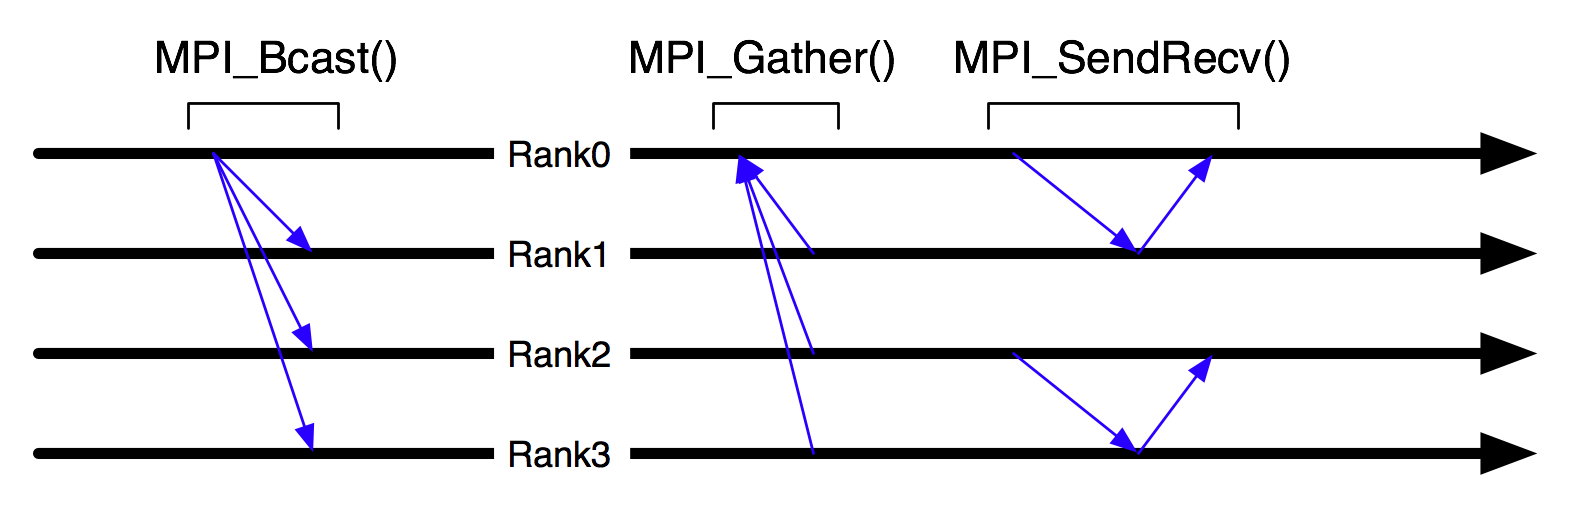
\includegraphics[height=1.5in]{mpi}\end{center}
    \note {MPI-All processes (normally one cpu per proccess but could be more) execute the same code. 
           These processes only know 'who they are' (their Rank). These ranks then have to explicitly 
           pass data.  This passing follows the form:
            \begin{enumerate}
              \item{Process 1 'Send to process 2'}
              \item{Process 2 'Recv from process 1'}
            \end{enumerate}
              \par Others options Colectives: \\ 
               \begin{itemize}
                \item {All process in a single Communicator,  'ALL DO THIS'}
               \end{itemize}
    }
  \end{frame}
  \begin{frame}{OpenMP}
   \begin{center}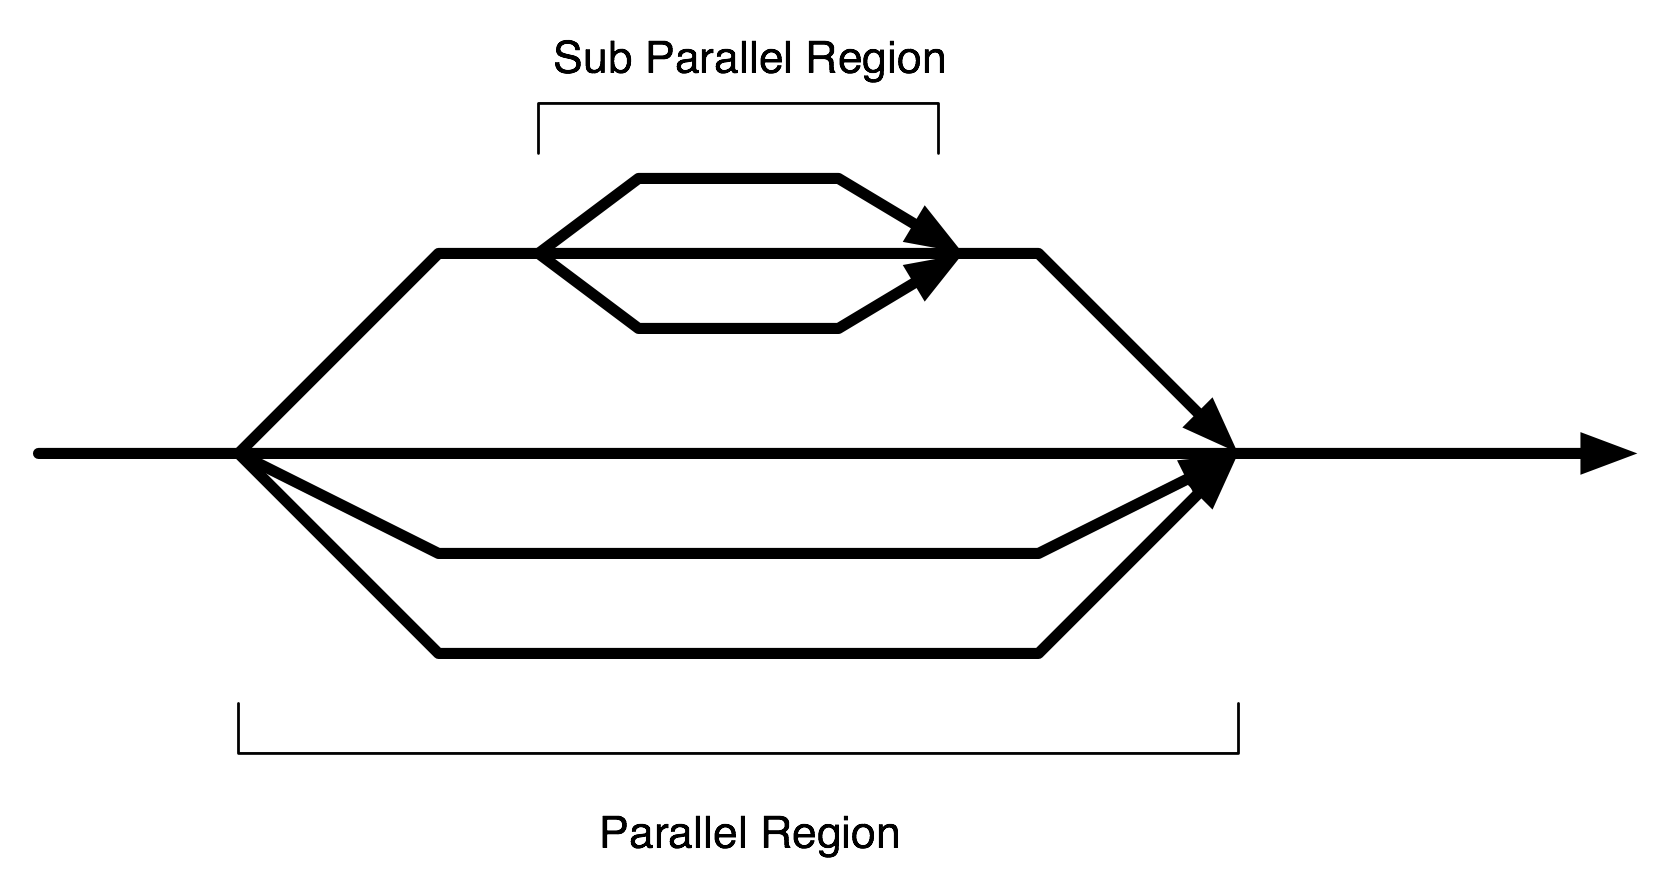
\includegraphics[height=2.5in]{openmp}\end{center}
   \note{OpenMP \url{http://www.openmpi.org} (Not to be confused with OpenMPI) is
         implimented in the compiler. Each compiler has its own issues with their 
         own implimentation of OpenMP but most users should find no problems with the basics.
         \begin{itemize}
           \item Anything that uses \texttt{OMP\_NUM\_THREADS} uses OpenMP
           \item PGI Compilers: \texttt{pgf90 -mp openmp.f90}
           \item Intel Compilers: \texttt{ifort -openmp openmp.f90}
         \end{itemize}
   }
  \end{frame}
  \begin{frame}{Other Options}
    \begin{block}{Other Options}
     \begin{itemize}
      \item<1->HPF-High Performance Fortran -- Use OpenMP/MPI
       \note[item]{HPF, \url{http://hpff.rice.edu/}}
      \item<2->pthreads -- Use OpenMP
       \note[item]{pthreads, \url{http://en.wikipedia.org/wiki/POSIX\_Threads}}
      \item<3->PVM -- Dead, Not installed, Use MPI
       \note[item]{PVM,\url{http://www.csm.ornl.gov/pvm/}}
      \item<4->CoArray
       \note[item]{CoArray, \url{http://www.co-array.org/}}
      \item<4-> Shmem -- Use \texttt{MPI\_Get()} and \texttt{MPI\_Put()}
       \note[item]{Shmem, \url{http://www.sgi.com/products/software/mpt/}}
     \end{itemize}
    \end{block}
  \end{frame}

  \section{Code}
   \subsection{Mechanics}
   \begin{frame}{MPI Mechanics}
    \begin{block}{Parts of an MPI Message}
     \begin{itemize}
     \item<1->{ Address of data, called a buffer}
     \item<1->{ MPI Datatype}
     \item<1->{ Count, or number of MPI datatypes to message}
     \item<2->{ Tag, Used to seperate messages from the same processor}
     \item<3->{ Communicator}
     \item<4->{ Rank of target}
     \end{itemize}
    \end{block}
    \note{
     MPI uses the buffer address, datatype and count to find how much raw data to send.
     For example, if MPI\_DOUBLE is 8 bytes, and count is 10, MPI 'knows' to send 80 bytes (10*8bytes) to the target process.  \\
     Note that \texttt{std::vector} is not a valid buffer for MPI! (or any STL class).  The STL does not make sure that all memory in continous. This breaks MPI, remember all buffers must be well defined. 

  } %end note
   \end{frame}
  \subsection{Utility Functions}
  \begin{frame}[fragile]
  \frametitle{MPI\_Init() MPI\_Finallize()}
   \begin{columns}[T]
    \begin{column}{5cm}
     \begin{block}{C}
      \begin{semiverbatim}
MPI\_Init(int  *argc,
          char ***argv)

MPI\_Finalize()
      \end{semiverbatim}
     \end{block}
    \end{column}
    \begin{column}{5cm}
     \begin{block}{Fortan}
      \begin{semiverbatim}
INTEGER IERROR
MPI\_INIT(IERROR)

MPI\_FINALIZE(IERROR)
      \end{semiverbatim}
     \end{block}
    \end{column}
   \end{columns}
   \begin{itemize}
     \item<2-> MPI\_Init() and MPI\_Finalize() should only be called once
     \item<3-> No other MPI calls are valid outside these functions
   \end{itemize}
\end{frame}

\end{document}
